%!TEX root = ../main.tex
\section{Lakebrain optimization} 
\label{sec:lakebrain}

Optimizing  query processing over large-scale data is significant in data warehouse and big data systems, as discussed in~\cite{}. However, for the \sys system with
complicated storage-disaggregated architecture with  multiple compute engines, it is challenging to optimize the end-to-end performance and resource usage. The reasons are two-fold. First, it is hard to capture the entire environment about the compute and storage cluster as well as the queries executed by other engines simultaneously. Second, even though all the environment data is available, it is still hard to optimize because of the large search space due to the large number of tunable and interdependent variables~\cite{}.

\cc{Do we address the first challenge ???}


To address the challenges, we present~\brain, a novel data lake storage optimizer that complements end-to-end data pipeline optimization. Unlike query engine optimizers that focus on join ordering and cardinality estimation~\cite{}, \brain aims to optimize data usage in storage~\cc{Then where is the performance?} during query execution, which is key to improve both query performance and storage resource utilization in a storage-disaggregated design.

\cc{Do you really design to achieve e2e optimization? what is the intuition of e2e?}

On the one hand, in a streaming application scenario, data ingestion and transactions often result in numerous small files, leading to low query performance on merge-on-read (MOR)\footnote{@} tables. Typical methods always \cc{XXX}.
 \brain  designs the automatic compaction (Section~\ref{subsec:compaction}) to combine these small files into fewer and larger ones, so as to  improve inter-cluster storage and network usage as well as query performance~\footnote{messy, query performance, storage resource, which one?}.

\cc{Below is very hard to follow! what is talking about?where is the partition? what is the connection with the above?}

On the other hand, with the data volume increasing, we  have to partition the data into different storage blocks such that the query efficiency can be much improved. In practice, users always select a single (or multiple) column as the partition key,  apply   a hash function to the values of the key, and then distribute the data to different blocks based on the partition values. This method is sub-optimal $w.r.t.$ the latency because it may lead to imbalanced data distribution. \brain  designs predicate-aware  method to partition the data in a fine-grained way such that given a query, the number of blocks to be assessed is minimized, and thus the efficiency is improved. (Section~\ref{subsec:partition})


%LakeBrain's design is kept simple for ease of extension and support for different applications. It consists of three components: a statistics collector, the core optimization logic, and an executor. The statistics collector gathers system configurations, environment variables, and workload history, while the core optimization logic employs heuristic rules, probabilistic models, and machine learning algorithms to suggest the best strategy candidates. The executor then deploys the chosen strategy, with its effects being collected as feedback by the statistics collector for future optimization.

Next, we will illustrate the above aspects in detail.

%To demonstrate the value of a data lake storage optimizer, we have developed two LakeBrain applications: auto compaction and predicate-aware fine-grained partitioning. These use cases will be explained in detail in the following section.

\subsection{Automatic Compaction}~\label{subsec:compaction}

As discussed above, file compaction aims to find the optimal strategy for compacting files that can improve query execution time or increased block utilization\footnote{not mentioned above} in storage. To achieve this goal, the optimization process employs two algorithms\footnote{two algorithms or steps?}: particle swarm optimization (PSO)\footnote{is there a citation? } and reinforcement learning (RL).

PSO is used to search for the global optimum, a population-based method that doesn't require assumptions about the relationship between tunable parameters and query performance. The goal is to obtain an approximately optimal solution within a limited time.  \cc{Not clear!! We should say what is the entire problem, and why and how to split it into two steps.}


\cc{Also not clear!! We should introduce what is the problem and the optimization goal that fit the paradigm of RL. Then define the critical components of RL and illustrate that.}
RL secondly finds a more sophisticated policy based on the states of the data lake environment.
The optimization process involves considering a set of discrete compaction configurations within the action space. Since the state space is continuous, a function approximation method is preferred. The stability of the training process is critical due to the high degree of variability in query performance in a distributed environment, so proximal policy optimization (PPO) is applied.

\begin{figure}[htbp]
	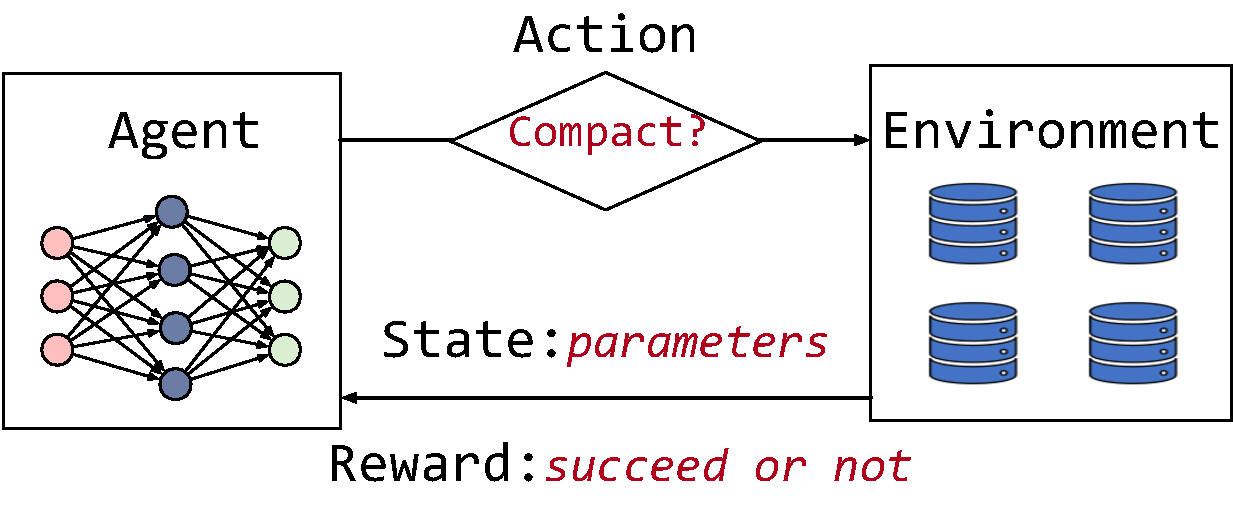
\includegraphics[scale=0.35]{figures/rl}
	\centering
	\vspace{-1em}
	\caption{Automatic Compaction using RL.}
	\label{fig:rl}
	\vspace{-1em}
\end{figure}

A deep neural network (DNN) is used to approximate the policy and the value function, with a shared feature backbone network that covers both global and local characteristics of the states. The output from the feature network is processed by two fully connected networks to compute the policy output and the action value. The actor and critic are alternatively updated after collecting new trajectories using the latest policy during training.

Once a desired result is obtained, the numerical output of the compaction strategy is translated into actionable operations by the data lake connector for a specific data lake engine, facilitating the optimization process.





\subsection{Predicate-aware Partitioning}~\label{subsec:partition}

Optimizing data partitioning~\footnote{* we should first say what is the data partition problem (does the previous section mention it?)} involves assigning records to storage blocks in the most efficient manner possible, thereby reducing the number of blocks accessed during queries. Our partitioning approach is based on the query-tree framework [43], and utilizes a sum-product network (SPN) probabilistic model [19, 26, 31] to model the distribution of the data in LakeBrain. This is done in order to ensure fast inference speed and avoid repeatedly scanning the datasets.

\cc{The high level idea of query-tree framework and spn should be introduced.}

\cc{how to leverage the distribution and why?}

The query-tree framework creates a tree-based partitioning strategy using pushdown predicates. Each leaf node represents a partition, and its column ranges are derived from the pushdown predicates used to split its parent nodes.
 By using probabilistic models to characterize the dataset, we can identify the most suitable partitioning policy. The probabilistic model-based cardinality estimation, as demonstrated in Figure 11, is used to estimate the number of records in each partition, \cc{How?? query-driven or data-driven? both cases should have queries to test} instead of scanning the original data, thereby saving a significant amount of time. This greatly improves the speed of the partitioning optimization algorithm, making it suitable for large-scale systems.

Additionally, probabilistic models allow us to represent a sequence of datasets with a series of probabilistic models that have a fixed structure but varying parameters. This is achieved by representing a sequence of datasets as a series of multi-dimensional vectors, each representing the learnable variables in the probabilistic model with a fixed length, i.e. a time series. We can then use time series prediction methods to predict future probabilistic models, and use these predictions to estimate the number of records in a partition during partitioning optimization\cc{like a magic}.


\begin{figure}[htbp]
	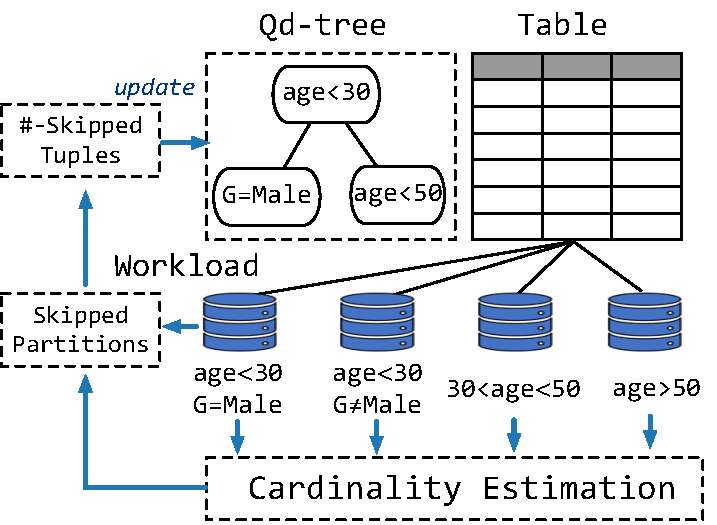
\includegraphics[scale=0.6]{figures/partition}
	\centering
	\vspace{-1em}
	\caption{Predicate-aware Partitioning.}
	\label{fig:partition}
	\vspace{-1em}
\end{figure}


\cc{Not coherent with the Next!}

To implement the optimized data layout, we introduce a partitioning mechanism that saves data in fine-grained partitions based on the partitioning strategy. Additionally, we have implemented an evaluator that skips irrelevant partitions by checking the overlap between pushdown predicates and the column ranges in each partition. For numerical columns, the range can be represented as lower and upper bounds, which are well-handled by many data formats. For categorical columns, we either record its range or its complement using "IN" or "NOT IN" predicates. The effectiveness of this predicate-aware partitioning approach is evaluated in section 7.2, where the test results show exceptional performance.
